\chapter{General framework} \label{s:fra}

\minitoc

\section{Introduction}

This chapter presents succinctly the spacetime framework used in these lectures
(Sec.~\ref{s:fra:spacetime})
and recalls useful basic concepts, such as worldlines of particles and observers
(Sec.~\ref{s:fra:worldlines} and \ref{s:fra:measure}).
In most of these lectures, we shall assume that the theory of gravitation is general
relativity; this means that the spacetime metric obeys Einstein equation,
which is recalled in Sec.~\ref{s:fra:Einstein_eq}.

This chapter is by no means an introduction to general relativity. We
recommend the textbooks \cite{Carro04,Choqu15,Hartl03,MisneTW73,Strau04,Wald84} in this
respect, as well as \cite{DerueU14,Gourg14,Langl13} for the French-speaking reader.

\section{Spacetime} \label{s:fra:spacetime}

In these lectures we consider a $n$-dimensional \defin{spacetime}\index{spacetime},
i.e. a pair $(\M, \w{g})$, where $\M$ is a $n$-dimensional smooth manifold, with $n\geq 2$, and $\w{g}$ is a Lorentzian metric on $\M$. In many parts, $n$ will be set to 4
--- the standard spacetime dimension --- but we shall also consider spacetimes with
$n>4$, especially in Chap.~\ref{s:hid}.

The precise definition and basic properties of a \emph{smooth manifold} are recalled
in Appendix~\ref{s:bas}. Here let us simply say that, in loose terms,
a \defin{manifold}\index{manifold} $\M$ of dimension $n$ is a ``space'' that \emph{locally} resembles $\R^n$,
i.e. can be described by a $n$-tuple of coordinates $(x^1,\ldots,x^n)$. However, globally,
$\M$ can be very different from $\R^n$, in particular regarding its topology.

\begin{figure}
\centerline{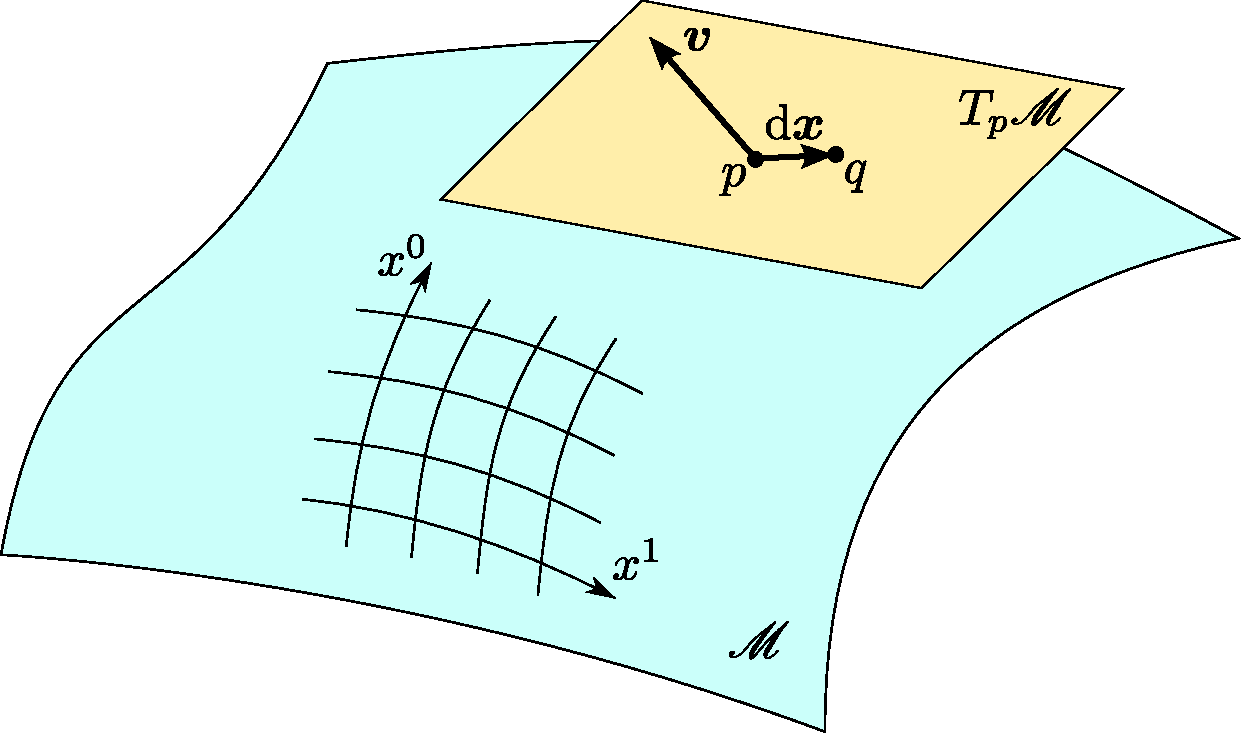
\includegraphics[width=0.6\textwidth]{fra_manifold.pdf}}
\caption[]{\label{f:fra:manifold} \footnotesize
A smooth manifold $\M$: the infinitesimal vector $\D\w{x}$ connects the nearby points $p$ and $q$ and thus
can thought as a displacement within the manifold, while the finite vector $\w{v}$ does not correspond to
any displacement in the manifold and ``lives'' in the tangent space $T_p\M$.}
\end{figure}


The smooth structure endows the manifold
with the concept of infinitesimal vectors\index{vector!infinitesimal --} $\D\w{x}$, which connect infinitely
close points of $\M$ (cf. Fig.~\ref{f:fra:manifold} and Sec.~\ref{s:bas:vectors} of Appendix~\ref{s:bas}). However, for finitely separated points, there is no
longer the concept of connecting vector (contrary for instance to points in $\R^n$).
In other words, vectors on $\M$ do not live in the manifold but in the
\defin{tangent spaces}\index{tangent!space} $T_p\M$, which are defined at each point $p\in\M$. Each  $T_p\M$
is a $n$-dimensional vector space, which is generated for instance by the infinitesimal displacement
vectors along the $n$ coordinate lines of some coordinate system.

The full definition of the \defin{metric tensor} $\w{g}$ is given in Sec.~\ref{s:bas:pRiemManif} of
Appendix~\ref{s:bas}. At each point $p\in\M$, $\w{g}$ induces a (non positive definite)
scalar product on $T_p\M$, which we shall denote by a dot:
\be
    \forall (\w{u},\w{v})\in T_p\M\times T_p\M, \quad
        \w{u}\cdot\w{v} := \w{g}(\w{u}, \w{v}) .
\ee
The fact that its signature is Lorentzian, i.e.
\be
\mathrm{sign}\; \w{g} = (-,\underbrace{+,\ldots,+}_{\mbox{\small $n-1$ times}}),
\ee
implies that from each point $p\in\M$, there are privileged directions,
which form the so-called \defin{null cones}\index{null!cone}
or \defin{light cones}\index{light:cone} (cf. Fig.~\ref{f:fra:lorentz_manifold} ).
The null cones constitute an absolute structure of spacetime, independent from any observer.

\begin{figure}
\centerline{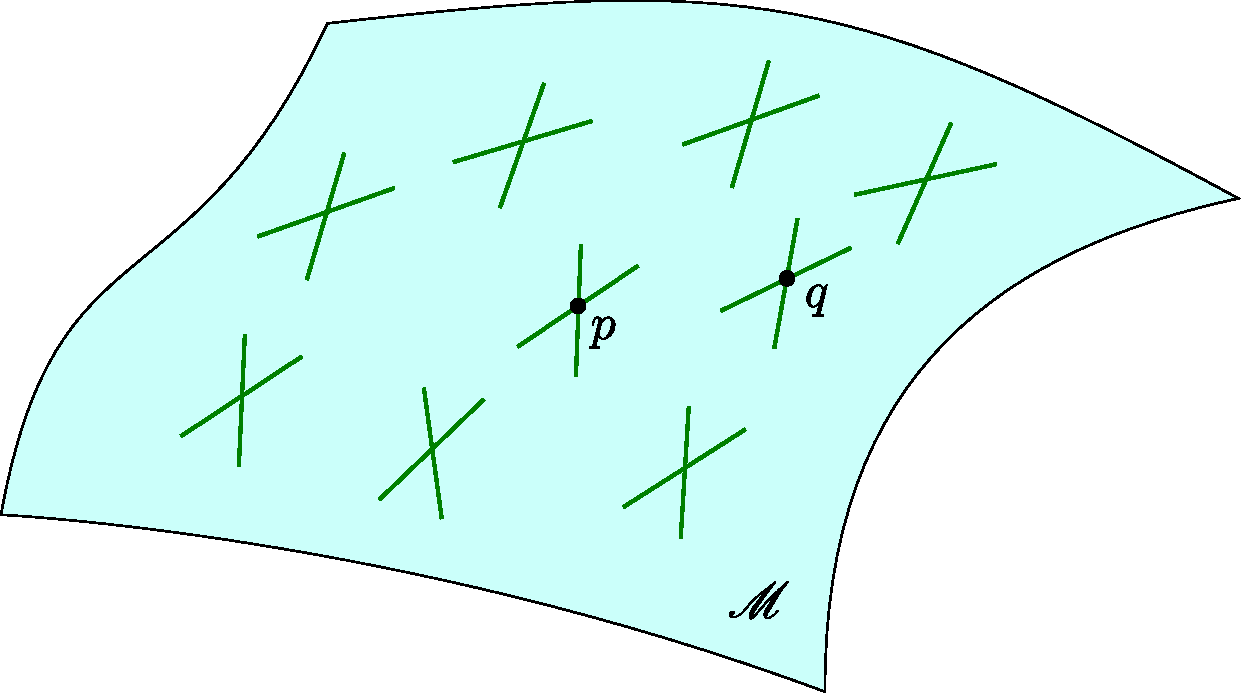
\includegraphics[width=0.6\textwidth]{fra_lorentz_manifold.pdf}}
\caption[]{\label{f:fra:lorentz_manifold} \footnotesize
A Lorentzian manifold $(\M,\w{g})$: at each point, the metric tensor $\w{g}$
defines priviledged directions: those lying in the null cone at $p$.}
\end{figure}



Unless explicitly specified, we assume that $\M$ is an orientable manifold (cf. Sec.~\ref{s:bas:Levi-Civita_tensor})
and that $(\M, \w{g})$ is time-orientable. The qualifier \defin{time-orientable}\index{time-orientable}\index{orientable!time --} means that it is possible to divide
\emph{continuously}
all non-spacelike vectors into two classes, which are called
\defin{future-directed}\index{future-directed} and \defin{past-directed}\index{past-directed}.
More precisely, at each tangent space $T_p\M$, let us split the non-spacelike
(i.e. timelike or null) vectors
in two classes, based on the equivalence relation
\[
  \w{u}\sim \w{v} \iff \w{g}(\w{u},\w{v}) \leq 0 .
\]
In loose terms, $\w{u}\sim \w{v}$ iff $\w{u}$ and $\w{v}$ are located inside
or onto the same sheet of the null cone at $p$.
$(\M,\w{g})$ is then time-orientable iff some choice of an equivalence class
can be performed continuously over the entire manifold $\M$.


\section{Worldlines} \label{s:fra:worldlines}

In relativity, a particle is described by its spacetime extent, which is a smooth curve,
$\Li$ say, and not a point. This curve is called the particle's
\defin{worldline}\index{worldline} and might be thought of as the set of
the ``successive positions'' occupied by the particle as ``time evolves''.
Except for pathological cases (tachyons\index{tachyon}),
the worldline has to be a \defin{causal curve}\index{causal!curve}\index{curve!causal --}, i.e.
at any point, a tangent vector to $\Li$  is either timelike or null.
This reflects the impossibility for the particle to travel faster than light with respect
to any local inertial frame.
The dynamics of a simple particle (i.e. a particle without any internal structure nor
spin) is entirely described by its
\defin{4-momentum}\index{4-momentum} or \defin{energy-momentum vector}\index{energy-momentum!vector}\footnote{When $n\not=4$, \emph{energy-momentum vector} is definitely a better name
than \emph{4-momentum}!}, which is a vector field $\w{p}$ defined along $\Li$,
tangent to $\Li$ at each point and future-directed (cf. Fig.~\ref{f:fra:worldline}).

\begin{figure}
\centerline{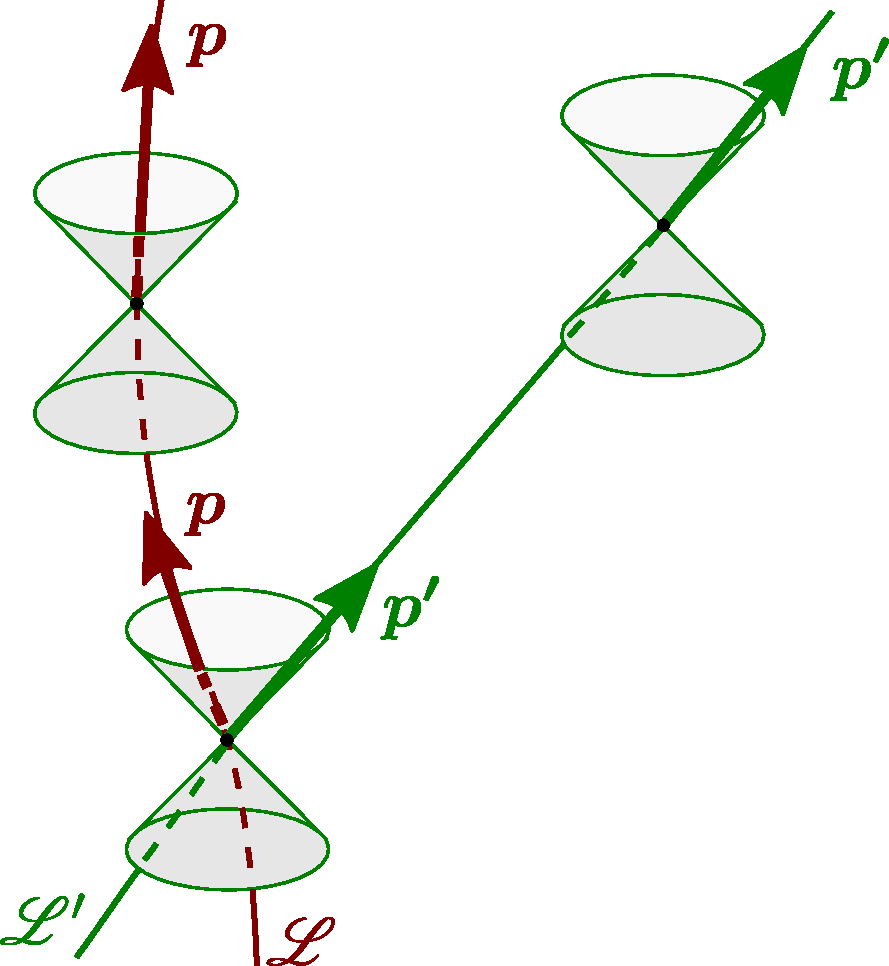
\includegraphics[width=0.4\textwidth]{fra_worldline.pdf}}
\caption[]{\label{f:fra:worldline} \footnotesize
Worldlines of a massive particle ($\Li$) and of a massless one ($\Li'$).}
\end{figure}


One distinguishes two types of particles:
\begin{itemize}
\item the \defin{massive particles}\index{massive!particle}\index{particle!massive --}, for which
$\Li$ is a timelike curve, or equivalently, for which
$\w{p}$ is a timelike vector:
\be
    \w{g}(\w{p},\w{p}) = \w{p}\cdot\w{p} < 0 ;
\ee
\item the \defin{massless particles}\index{massless!particle}\index{particle!massless --},
such as the photon,
for which $\Li$ is a null curve, or equivalently, for which  $\w{p}$ is a null vector:
\be
    \w{g}(\w{p},\w{p}) = \w{p}\cdot\w{p} = 0 .
\ee
\end{itemize}
In both cases, the \defin{mass} of the particle is defined by\footnote{Unless specified, we use geometrized units, for which $G=1$ and $c=1$.}
\be \label{e:fra:def_mass}
   m = \sqrt{- \w{p}\cdot\w{p}} .
\ee
Of course, for a massless particle, we get $m=0$.

If the particle feels only gravitation, i.e. if no non-gravitational force
is exerted on it, the energy-momentum vector must be a
\defin{geodesic vector}\index{geodesic!vector}, i.e. it obeys
\be \label{e:fra:p_geodesic}
    \encadre{\wnab_{\w{p}}\,  \w{p} = 0 } ,
\ee
or, in index notation,
\be
    p^\mu \nabla_\mu p^\alpha = 0 .
\ee
This implies that the worldline $\Li$ must be a
\defin{geodesic}\index{geodesic} of the spacetime $(\M,\w{g})$.
\begin{remark} \label{r:fra:geodesic_vector}
The reverse is not true, i.e. having $\Li$ geodesic and $\w{p}$
tangent to $\Li$ does not imply (\ref{e:fra:p_geodesic}), but the
weaker condition $\wnab_{\w{p}}\,  \w{p} = \alpha \, \w{p}$, with $\alpha$
a scalar field along $\Li$. In this case, one says that $\w{p}$ is a
\defin{pregeodesic vector}\index{pregeodesic!vector}.
\end{remark}
For massive particles, Eq.~(\ref{e:fra:p_geodesic}) can be derived from
a variational principle, the action being simply the worldline's length
as given by the metric tensor:
\be
    S = \int_A^B \D s = \int_{\lambda_A}^{\lambda_B}
     \sqrt{-\w{g}\left(\frac{\D\w{x}}{\D\lambda}, \frac{\D\w{x}}{\D\lambda} \right)}
     \, \D\lambda .
\ee
For photons, Eq.~(\ref{e:fra:p_geodesic}) can be derived from the Maxwell equations
within the geometrical optics approximation, with the assumption that
the photon energy-momentum vector is related to the wave 4-vector $\w{k}$ by
\be \label{e:fra:p_hbar_k}
    \w{p} = \hbar \w{k} .
\ee

\subsection{Massive particles}

For a massive particle, the constraint of having the worldline $\Li$ timelike
has a simple geometrical meaning: $\Li$ must
always lie inside the light cones of events along $\Li$ (cf. Fig.~\ref{f:fra:worldline}).
The fundamental link between physics and geometry is that the
\defin{proper time}\index{proper!time}\index{time!proper --} $\tau$ of the particle
is nothing but the metric length along the worldline, increasing towards the future:
\be \label{e:fra:proper_time}
    \D\tau = \sqrt{- \w{g}(\D\w{x}, \D\w{x})} = \sqrt{- g_{\mu\nu} \D x^\mu \, \D x^\nu} ,
\ee
where $\D\w{x}$ is an infinitesimal future-directed displacement
along $\Li$.

The particle's \defin{4-velocity}\index{4-velocity} is defined the
derivative vector $\w{u}$ of the parametrization of
$\Li$ by the proper time:
\be \label{e:fra:def_u}
    \encadre{ \w{u} := \frac{\D\w{x}}{\D\tau} }.
\ee
By construction, $\w{u}$ is tangent to $\Li$ and is a unit timelike vector:
\be \label{e:fra:u_unit}
    \w{u}\cdot\w{u} = -1 .
\ee
For a simple particle (no internal structure),
the 4-momentum $\w{p}$ is tangent to $\Li$; it is then necessarily
collinear to $\w{u}$. Since both vectors are future-directed,
Eqs.~(\ref{e:fra:def_mass}) and (\ref{e:fra:u_unit}) lead to
\be \label{e:fra:p_m_u}
    \w{p} = m\, \w{u} .
\ee

\subsection{Massless particles (photons)}

For a massless particle, Eq.~(\ref{e:fra:proper_time}) would lead to $\D\tau=0$
since the displacement $\D\w{x}$ would be a null vector. There is then no natural parameter
along a null geodesic. However, one can single out a whole family of them,
called \emph{affine parameters}. An \defin{affine parameter}\index{affine!parameter}
along a null geodesic $\Li$ is a parameter $\lambda$ such that
the associated tangent vector,
\be
    \w{v} := \frac{\D\w{x}}{\D\lambda} ,
\ee
is a geodesic vector field: $\wnab_{\w{v}} \, \w{v} = 0$. In general,
the tangent vector associated to a given parameter fullfils only
$\wnab_{\w{v}} \, \w{v} = \alpha \, \w{v}$, with $\alpha$ a scalar field
along $\Li$ (cf. Remark~\ref{r:fra:geodesic_vector} above).

The qualifier \emph{affine} arises from the fact any two affine parameters
$\lambda$ and $\lambda'$ are related by an affine transformation:
\be \label{e:fra:affine_transf}
    \lambda' = a \lambda + b,
\ee
with $a$ and $b$ two constants.
Given that the photon energy-momentum vector $\w{p}$ is a geodesic vector
[Eq.~(\ref{e:fra:p_geodesic})],
a natural choice of the affine parameter $\lambda$ is that associated with
$\w{p}$:
\be \label{e:fra:p_dxdl}
    \w{p} = \frac{\D\w{x}}{\D\lambda} .
\ee
This fixes $a=1$ in the transformation (\ref{e:fra:affine_transf}).


\begin{figure}
\centerline{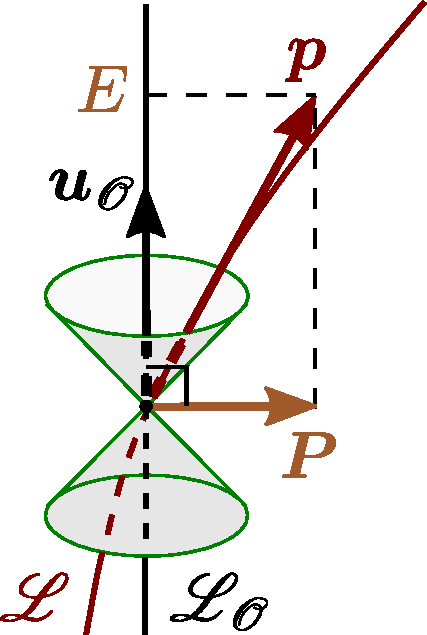
\includegraphics[height=0.3\textheight]{fra_energy_momentum.pdf}}
\caption[]{\label{f:fra:energy_momentum} \footnotesize
Orthogonal decomposition of the energy-momentum vector $\w{p}$ of a particle
with respect to the 4-velocity $\w{u}_{\Obs}$ of an observer $\Obs$,
giving birth to the energy $E$ and linear momentum $\w{P}$ as measured by $\Obs$.}
\end{figure}



\section{Quantities measured by an observer} \label{s:fra:measure}

In the simplest modelization, an \defin{observer}\index{observer} $\Obs$
is described by a timelike worldline $\Li_{\Obs}$ in the spacetime $(\M,\w{g})$.
Let us suppose that the observer encounters a particle at some event $A$.
Geometrically, this means that the worldline $\Li$ of the particle
intersects $\Li_{\Obs}$ at $A$. Then, the \defin{energy}\index{energy!of a particle}
$E$ and the \defin{momentum}\index{momentum!of a particle} $\w{P}$ of the
particle, both measured by $\Obs$, are given by the orthogonal decomposition of the
particle's energy-momentum vector $\w{p}$ with respect to $\Li_{\Obs}$
(cf. Fig.~\ref{f:fra:energy_momentum}):
\be \label{e:fra:p_E_P}
    \encadre{ \w{p} = E \w{u}_{\Obs} + \w{P} },\quad\mbox{with}\quad
        \w{u}_{\Obs}\cdot\w{P} = 0 ,
\ee
where $\w{u}_{\Obs}$ is the 4-velocity of observer $\Obs$, i.e. the future-directed
unit tangent vector to $\Li_{\Obs}$.
By taking the scalar product of Eq.~(\ref{e:fra:p_E_P}) with $\w{u}_{\Obs}$,
we obtain the following expressions for $E$ and $\w{P}$:
\be \label{e:fra:E_obs}
    \encadre{E = - \w{u}_{\Obs}\cdot\w{p}}
\ee
\be
    \encadre{\w{P} = \w{p} + (\w{u}_{\Obs}\cdot\w{p})\, \w{u}_{\Obs}} .
\ee
The scalar square of Eq.~(\ref{e:fra:p_E_P}) leads to
\be
    \underbrace{\w{p}\cdot\w{p}}_{-m^2} = E^2
    \underbrace{\w{u}_{\Obs}\cdot\w{u}_{\Obs}}_{-1} + 2 E \underbrace{\w{u}_{\Obs}\cdot\w{P}}_{0}
    + \w{P}\cdot\w{P} ,
\ee
where we have used Eq.~(\ref{e:fra:def_mass}) to let appear the particle's mass
$m$. Hence we recover Einstein's relation\index{Einstein!relation}:
\be \label{e:fra:E2_m2_P2}
    \encadre{E^2 = m^2 + \w{P}\cdot\w{P} }.
\ee

An infinitesimal displacement $\D\w{x}$ of the particle along its worldline
is related to the energy-momentum vector $\w{p}$ by
\be \label{e:fra:dx_p_dl}
    \D\w{x} = \w{p} \, \D\lambda,
\ee
where $\lambda$ is the affine parameter along the particle's worldline
whose tangent vector is $\w{p}$ [cf. Eq.~(\ref{e:fra:p_dxdl}) for a massless
particle and Eqs.~(\ref{e:fra:def_u}) and (\ref{e:fra:p_m_u}) with
$\lambda := \tau/m$ for a massive particle]. Substituting (\ref{e:fra:p_E_P})
for $\w{p}$ in (\ref{e:fra:dx_p_dl}), we get the orthogonal decomposition
of $\D\w{x}$ with respect to $\Li_{\Obs}$:
\be
    \D\w{x} = E \D\lambda \, \w{u}_{\Obs} + \D\lambda\,  \w{P} .
\ee
$\Obs$'s proper time elapsed during the particule displacement is the
coefficient in front of $\w{u}_{\Obs}$: $\D\tau_{\Obs} = E \D\lambda$ and the
the particle's displacement in $\Obs$'s rest frame is the part orthogonal
to $\w{u}_{\Obs}$: $\D\w{X} = \D\lambda\,  \w{P}$. By definition,
the particle's velocity with respect to $\Obs$ is
\be
    \w{V} := \frac{\D\w{X}}{\D\tau_{\Obs}} = \frac{\D\lambda\,  \w{P}}{E \D\lambda}.
\ee
Hence the relation
\be \label{e:fra:P_E_V}
    \encadre{ \w{P} = E \, \w{V}} .
\ee

Relations (\ref{e:fra:E2_m2_P2}) and (\ref{e:fra:P_E_V}) are valid for any kind of particle, massive or not.
For a massive particle, the energy-momentum vector $\w{p}$ is related to the
particle's 4-velocity $\w{u}$ via (\ref{e:fra:p_m_u}). Inserting this relation
into (\ref{e:fra:E_obs}), we obtain
\be \label{e:fra:E_Gam_m}
    E = \Gamma \, m,
\ee
where
\be
    \Gamma := - \w{u}_{\Obs}\cdot\w{u}
\ee
is the \defin{Lorentz factor}\index{Lorentz!factor} of the particle with respect
to the observer. If we depart from units with $c=1$, Eq.~(\ref{e:fra:E_Gam_m})
becomes the famous relation $E = \Gamma m c^2$.
Combining (\ref{e:fra:P_E_V}) and (\ref{e:fra:E_Gam_m}) yields also a familiar
relation:
\be \label{e:fra:P_Gam_m_V}
    \w{P} = \Gamma m \, \w{V} .
\ee
Finally, inserting (\ref{e:fra:E_Gam_m}) and (\ref{e:fra:P_Gam_m_V}) into
(\ref{e:fra:E2_m2_P2}) leads to the well-known expression of the Lorentz factor in
terms of the velocity:
\be
    \Gamma = \left( 1 - \w{V}\cdot\w{V} \right) ^{-1/2} .
\ee

For a massless particle (photon), inserting (\ref{e:fra:P_E_V}) into the
Einstein relation (\ref{e:fra:E2_m2_P2}) with $m=0$ yields
\be
    \w{V}\cdot\w{V} = 1 .
\ee
This means that the norm of the velocity of the massless particle with respect to $\Obs$
is the speed of light $c$ ($=1$ in our units).
For a photon associated with a monochromatic radiation, the wave 4-vector $\w{k}$
admits the following orthogonal decomposition:
\be
    \w{k} = \omega \left(\w{u} + \w{V} \right) ,
\ee
where $\omega = 2\pi \nu$ and $\nu$ is the radiation frequency as measured by
observer $\Obs$. In view of (\ref{e:fra:p_hbar_k}) and (\ref{e:fra:p_E_P}), we
get the Planck-Einstein relation\index{Planck-Einstein relation}:
\be
    E = h \nu .
\ee

\section{Einstein equation} \label{s:fra:Einstein_eq}

Saying that gravitation in the spacetime $(\M, \w{g})$ is ruled by
\defin{general relativity}\index{general!relativity} amounts
to demanding that the metric $\w{g}$ obeys \defin{Einstein equation}\index{Einstein!equation}:
\be \label{e:bas:Einstein_eq}
    \encadre{ \w{R} - \frac{1}{2}\, R\, \w{g} + \Lambda\, \w{g} = 8\pi \w{T} },
\ee
where $\w{R}$ is the Ricci tensor of $\w{g}$, $R$ is the Ricci scalar of $\w{g}$
(cf. Sec.~\ref{s:bas:Ricci_tensor} in Appendix~\ref{s:bas}), $\Lambda$ is some
constant, called the \defin{cosmological constant}\index{cosmological!constant},
and $\w{T}$ is the energy-momentum tensor\index{energy-momentum tensor} of
matter and non-gravitational fields.

By taking the trace of (\ref{e:bas:Einstein_eq}) with respect to $\w{g}$, it is
easy to show that the Einstein equation (\ref{e:bas:Einstein_eq}) is
equivalent to
\be \label{e:bas:Einstein_eq_n}
    \encadre{ \w{R}  = \frac{2}{n-2}\,\Lambda\,  \w{g}
    + 8\pi \left( \w{T} - \frac{1}{n-2}\,  T \, \w{g} \right) },
\ee
where $T := g^{\mu\nu} T_{\mu\nu}$ is the trace of $\w{T}$ with respect to
$\w{g}$.

\begin{remark}
The dimension $n$ of the spacetime does not appear in the Einstein equation
(\ref{e:bas:Einstein_eq}); on the contrary, the variant
(\ref{e:bas:Einstein_eq_n}) depends on $n$.
\end{remark}
